% Figure 4: Non-Uniform Voltage Grid + ΔV-Weighted Metric
% Compile: pdflatex fig4_voltage_grid.tex
\documentclass[border=8pt]{standalone}
\usepackage{tikz}
\usepackage{amsmath,amssymb}
\usepackage{pgfplots}
\pgfplotsset{compat=1.18}
\usetikzlibrary{
  arrows.meta,
  calc,
  positioning,
  decorations.pathreplacing,
  patterns,
  backgrounds,
  shadows.blur
}

\definecolor{coarseblue}{HTML}{2980B9}
\definecolor{denseorange}{HTML}{E67E22}
\definecolor{annotgray}{HTML}{7F8C8D}
\definecolor{bgcard}{HTML}{FDFEFE}
\definecolor{eqnpurple}{HTML}{8E44AD}
\definecolor{gaussgrn}{HTML}{27AE60}
\definecolor{mppgold}{HTML}{F39C12}

\begin{document}
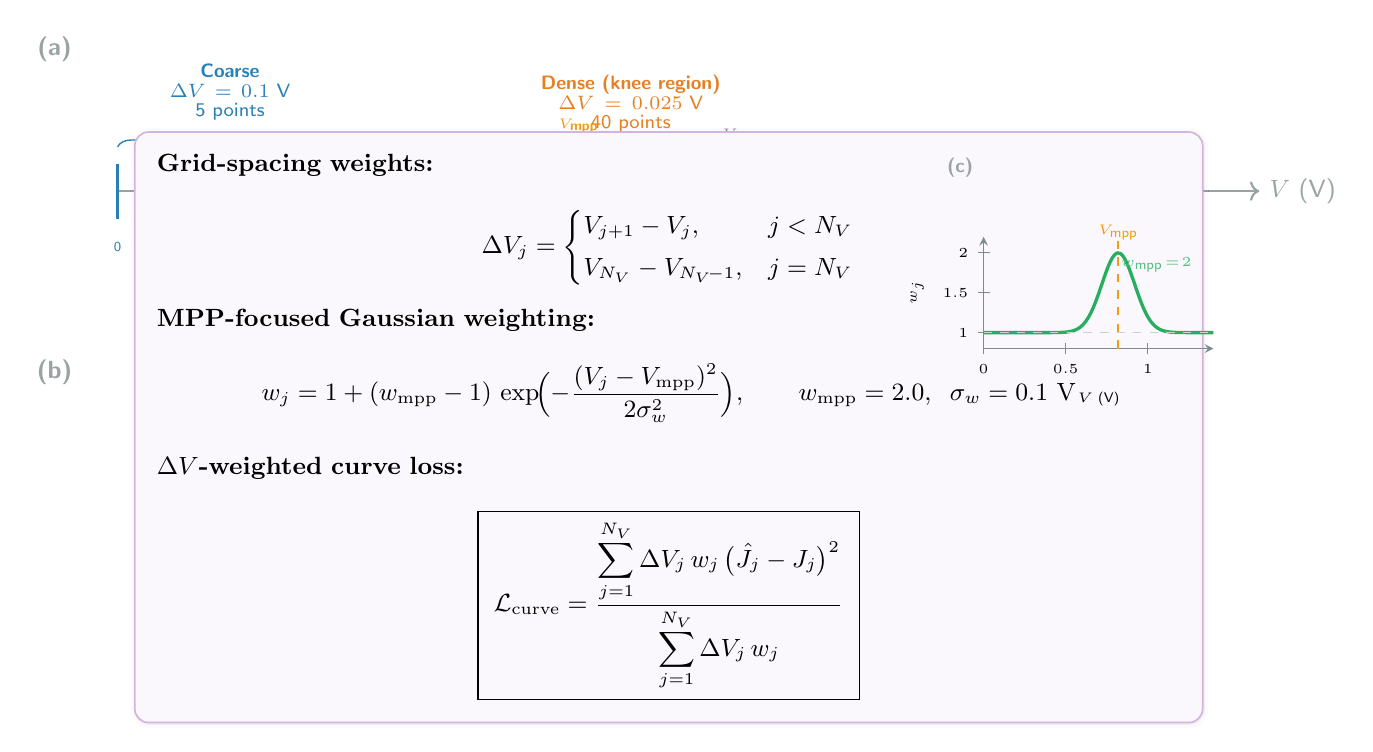
\begin{tikzpicture}[
  every node/.style={font=\sffamily\small},
  annot/.style={font=\sffamily\scriptsize, text=annotgray},
]

% ═══════════════════════════════════════════
% PANEL (a): Voltage Grid Axis
% ═══════════════════════════════════════════
\node[font=\sffamily\small\bfseries, text=annotgray!80] at (-0.8, 1.8) {(a)};

% Main axis line
\draw[->, line width=0.8pt, annotgray!80] (0, 0) -- (14.5, 0)
  node[right, font=\sffamily\small] {$V$ (V)};

% ─── Coarse region: 0 to 0.4 V (step 0.1) ───
% Positions: 0.0, 0.1, 0.2, 0.3, 0.4
% Scale: 10 cm per 1.4V → each 0.1V = ~0.714 cm
\pgfmathsetmacro{\scale}{10.0/1.4}

% Coarse ticks (all 5 drawn, labels at endpoints only)
\foreach \v in {0.0, 0.1, 0.2, 0.3, 0.4} {
  \pgfmathsetmacro{\xpos}{\v * \scale}
  \draw[coarseblue, line width=1.0pt] (\xpos, -0.35) -- (\xpos, 0.35);
}
% Labels at coarse endpoints
\node[below=5pt, font=\sffamily\tiny, text=coarseblue] at (0, -0.35) {0};
\node[below=5pt, font=\sffamily\tiny, text=coarseblue] at ({0.4*\scale}, -0.35) {0.4};

% Coarse region brace
\draw[
  decorate, decoration={brace, amplitude=5pt, raise=6pt},
  line width=0.5pt, coarseblue
] (0, 0.35) -- ({0.4*\scale}, 0.35)
  node[midway, above=12pt, font=\sffamily\scriptsize, text=coarseblue, text width=2cm, align=center] {
    \textbf{Coarse}\\[-1pt]
    $\Delta V = 0.1$ V\\[-1pt]
    5 points
  };

% ─── Dense region: 0.425 to 1.4 V (step 0.025) ───
% 40 ticks
\foreach \i in {0, 1, ..., 39} {
  \pgfmathsetmacro{\v}{0.425 + \i * 0.025}
  \pgfmathsetmacro{\xpos}{\v * \scale}
  \draw[denseorange, line width=0.5pt] (\xpos, -0.2) -- (\xpos, 0.2);
}

% Key labels in dense region
\pgfmathsetmacro{\xfour}{{0.425*\scale}}
\node[below=5pt, font=\sffamily\tiny, text=denseorange] at (\xfour, -0.2) {0.425};
\pgfmathsetmacro{\xone}{{1.0*\scale}}
\node[below=5pt, font=\sffamily\tiny, text=denseorange] at (\xone, -0.2) {1.0};
\pgfmathsetmacro{\xend}{{1.4*\scale}}
\node[below=5pt, font=\sffamily\tiny, text=denseorange] at (\xend, -0.2) {1.4};

% Dense region brace
\draw[
  decorate, decoration={brace, amplitude=5pt, raise=6pt},
  line width=0.5pt, denseorange
] ({0.425*\scale}, 0.2) -- ({1.4*\scale}, 0.2)
  node[midway, above=12pt, font=\sffamily\scriptsize, text=denseorange, text width=2.5cm, align=center] {
    \textbf{Dense (knee region)}\\[-1pt]
    $\Delta V = 0.025$ V\\[-1pt]
    40 points
  };

% Total count
\node[
  draw=annotgray!40, fill=bgcard, rounded corners=2pt,
  font=\sffamily\scriptsize, text=annotgray!90,
  inner sep=3pt
] at ({0.7*\scale}, -1.1) {
  $N_V = 45$ total evaluation points
};

% ─── Typical Vmpp marker ───
\pgfmathsetmacro{\xmpp}{{0.82*\scale}}
\draw[mppgold, line width=1.2pt] (\xmpp, -0.5) -- (\xmpp, 0.5);
\node[above=3pt, font=\sffamily\tiny\bfseries, text=mppgold] at (\xmpp, 0.5) {$V_{\text{mpp}}$};
% Typical Voc marker
\pgfmathsetmacro{\xvoc}{{1.1*\scale}}
\draw[annotgray, line width=0.8pt, dashed] (\xvoc, -0.4) -- (\xvoc, 0.4);
\node[above=3pt, font=\sffamily\tiny, text=annotgray] at (\xvoc, 0.4) {$V_{\text{oc}}$};

% ═══════════════════════════════════════════
% PANEL (b): ΔV-Weighted Loss Equation
% ═══════════════════════════════════════════
\node[font=\sffamily\small\bfseries, text=annotgray!80] at (-0.8, -2.3) {(b)};

\node[
  draw=eqnpurple!40,
  fill=eqnpurple!4,
  rounded corners=5pt,
  line width=0.6pt,
  text width=13cm,
  align=left,
  font=\small,
  inner sep=8pt,
  blur shadow={shadow blur steps=2, shadow xshift=0.3pt, shadow yshift=-0.3pt, shadow opacity=12}
] (eqnbox) at (7.0, -3.0) {
  \textbf{Grid-spacing weights:}
  \vspace{2pt}
  \[
    \Delta V_j =
    \begin{cases}
      V_{j+1} - V_j, & j < N_V \\[2pt]
      V_{N_V} - V_{N_V\!-1}, & j = N_V
    \end{cases}
  \]
  \vspace{-6pt}

  \textbf{MPP-focused Gaussian weighting:}
  \vspace{2pt}
  \[
    w_j = 1 + (w_{\text{mpp}} - 1)\,\exp\!\Bigl(-\frac{(V_j - V_{\text{mpp}})^2}{2\sigma_w^2}\Bigr),
    \qquad w_{\text{mpp}} = 2.0,\;\; \sigma_w = 0.1\text{ V}
  \]
  \vspace{-4pt}

  \textbf{$\Delta V$-weighted curve loss:}
  \vspace{2pt}
  \[
    \boxed{\;
    \mathcal{L}_{\text{curve}}
    = \frac{\displaystyle\sum_{j=1}^{N_V} \Delta V_j \, w_j \,
      \bigl(\hat{J}_j - J_j\bigr)^2}
      {\displaystyle\sum_{j=1}^{N_V} \Delta V_j \, w_j}
    \;}
  \]
};

% ═══════════════════════════════════════════
% PANEL (c): Gaussian weighting bump (mini plot)
% ═══════════════════════════════════════════
\begin{scope}[shift={(11.0, -2.0)}]
  \node[font=\sffamily\scriptsize\bfseries, text=annotgray!80] at (-0.3, 2.3) {(c)};

  \begin{axis}[
    width=4.5cm,
    height=3.0cm,
    at={(0cm,0cm)},
    anchor=south west,
    xlabel={$V$ (V)},
    ylabel={$w_j$},
    xlabel style={font=\sffamily\tiny},
    ylabel style={font=\sffamily\tiny},
    tick label style={font=\sffamily\tiny},
    xmin=0, xmax=1.4,
    ymin=0.8, ymax=2.2,
    axis lines=left,
    axis line style={line width=0.4pt, color=annotgray},
    every tick/.style={annotgray, line width=0.3pt},
    grid=none,
    clip=false,
  ]

  % Gaussian bump centered at Vmpp=0.82
  \addplot[
    gaussgrn, line width=1.2pt, smooth, samples=80, domain=0:1.4
  ] {1.0 + 1.0 * exp(-((x - 0.82)^2) / (2 * 0.1^2))};

  % Baseline w=1 line
  \addplot[annotgray!40, line width=0.4pt, dashed, domain=0:1.4] {1.0};

  % Vmpp marker
  \draw[mppgold, line width=0.8pt, dashed] (axis cs:0.82, 0.8) -- (axis cs:0.82, 2.15);
  \node[font=\sffamily\tiny, text=mppgold] at (axis cs:0.82, 2.25) {$V_{\text{mpp}}$};

  % w_mpp annotation
  \node[font=\sffamily\tiny, text=gaussgrn!80] at (axis cs:1.05, 1.85) {$w_{\text{mpp}}\!=\!2$};

  \end{axis}
\end{scope}

\end{tikzpicture}
\end{document}
